\documentclass[conference]{IEEEtran}
\IEEEoverridecommandlockouts
% The preceding line is only needed to identify funding in the first footnote. If that is unneeded, please comment it out.
\usepackage{cite}
%\usepackage{hyperref}
\usepackage{amsmath,amssymb,amsfonts}
\usepackage{algorithmic}
\usepackage{graphicx} \usepackage{textcomp}
\usepackage{xcolor, soul}
\sethlcolor{gray}
\usepackage{url}
\usepackage{caption}
\captionsetup[table]{skip=3pt}
\usepackage{cleveref}
\usepackage{subfiles}
\def\BibTeX{{\rm B\kern-.05em{\sc i\kern-.025em b}\kern-.08em
T\kern-.1667em\lower.7ex\hbox{E}\kern-.125emX}}
\begin{document}

    \title{Project 7: Studying ISIS Twitter influence with social network analysis from the pro-ISIS fanboy tweet data}
%{\footnotesize \textsuperscript{*}Note: Sub-titles are not captured in Xplore and
%should not be used}
%}




    \author{\IEEEauthorblockN{1\textsuperscript{st} Niklas Saari}
    \IEEEauthorblockA{\textit{dept. Computer Science and Engineering} \\
    \textit{University of Oulu}\\
    Oulu, Finland \\
    niklas.saari@student.oulu.fi}
    }

    \maketitle

    \begin{abstract}
        This document describes project work for the course Social Network Analysis in Spring 2021.
        Radical and extreme groups have taken social networks as part of their toolchain to spread propaganda messages,
        get attention, look support for their actions and recruit more members.
        One of the most brutal of these groups, ISIS, which is also designated as terrorist organization, has been forerunner on using these social platforms successfully.
        To possibly prevent future terror events, it would be important to study these social networks on how they are used by these radical groups.
        ISIS Twitter dataset of around 17~000 tweets was selected as dataset to identify important characters from the network, to construct communities and to see how the most influencers behave, who they are, and how they connect to other people.
        Further communities were constructed to see how networks behave internally.
        Initial results suggests that primal pro-ISIS fanboy accounts were identified, and they are using social networks efficiently to distribute messages by creating
        close communities with selected hashtags.

    \end{abstract}

    \begin{IEEEkeywords}
        Twitter, Social Network Analysis, Terrorism, Networks, ISIS
    \end{IEEEkeywords}


    \section{Group information}\label{sec:group-description}

    This project has been done alone.
    The original project from the given project list was 7 with the title of "Analysis of ISIS Twitter dataset".
    Project source code and also source code of this article can found from \href{https://github.com/Nicceboy/SNA-project-2021}


    \section{Introduction}\label{sec:introduction}

    Social networks have become part of the most people's everyday life.
    These networks, such as Facebook, Twitter or Reddit are base for many kinds of groups and people for communicating with each other.
    They are being used widely for expressing opinions or advertising services and for many other kinds of things.
    This has naturally risen special interest in radical and terrorism organisations because of the provided possibility for
    influencing different kind of people with a large scale.
    While the brutality of terrorism has become even more severe over recent time based on the data gathered by Global
    Terrorism Database and seen in Appendixes in the figure \ref{fig:appendix_terrorism_deaths}, this raises specific interest
    in terms of identifying and preventing possible future incidents.

    Terrorism is identified to be especially brutal from Islamic State of Iraq and Levant (ISIL), which is also known ISIS
    or Daesh.\cite{enwiki:1024074085}
    Their usage of the social media is also known to be "probably more sophisticated than [that of] most US companies",\cite{isis-selling-terror}
    and has been one of their main campaigning tactics in Syria and Iraq.
    Twitter has been their primal social network\cite{isis-how-twitter} so far.
    It is known that ISIS has been previously organising for example specific hashtag campaigns to get their topics
    trending and gain more visibility\cite{isis-how-twitter}.

    Because the social networks have begun to be in key role to motivate support for their actions, raise funds and even for recruiting
    foreign fighters with huge success\cite{isis-foreign-fighter} allowing organisation to reach worldwide recognition and impact,
    it is important to study how these networks are formed and what we could learn from them and how we could act based on this information.

    Social Network Analysis (SNA) is a process for studying social life by social structures which is constructed by relations and patterns formed by these relations.
    This is usually done with networks and applying the graph theory.\cite{marin2011social, doi:10.1177/016555150202800601}

    In this article we will focus particularly on the Twitter platform and for the Social Network Analysis of how ISIS has been using this specific
    platform to spread their propaganda and organizing recruitment.
    Twitter data of over 17~000 tweets of pro-ISIS fanboys has been used as dataset for this study.

    We will try to identify major characters from the provided data, for example which characters have the most influence and
    what kind of networks they are constructing.
    This is evaluated based on different values specific for Twitter platform, such as usage of mentions, retweets or hashtags; how are different Twitter users using them.

    We further try to estimate the sentiment of the tweets in terms of negative, neutral and positive and estimate the most
    frequent hashtags and their possible context and characteristics.
    Sentiments are finally plotted with ternary plots by different characteristics.
    Different kind of other graphs will be constructed to develop our understanding of underlying network.
    Social network is constructed by using hashtags, and their relations to other tweets based on their appearances.

    This document is structured as following: in the section~\ref{sec:problem-description} the main problem has been described.
    In the section~\ref{sec:dataset-description} the exact details of the used dataset has been described.
    In the section~\ref{sec:general-methodology} general methodology has been described and further continued in the section~\ref{sec:detailed-methodology}
    in more precise matter.
    The results are presented in the section~\ref{sec:results-and-discussion} and paper has been finally concluded in the section~\ref{sec:conclusion-and-perspectives}.


    \section{Problem Description}\label{sec:problem-description}

    The main problem is to study and tell how we can find specific communities from underlying dataset and identify interesting
    numerical values from the constructed network.
    Can we detect specific patterns or behaviours related to specific Twitter users, is there connection between them and how powerful their influence actually is?
    We further try to find a way to tell about what kind of messages they are distributing in overall.
    Dataset was not collected by itself, instead it was given in the project assignment.


    \section{Dataset description}\label{sec:dataset-description}

    Twitter dataset of tweets collected from pro-ISIS fanboys of all over the world has been used as a base for this study.
    This dataset was provided with the project assigment.
    Based on the same project assigment, the origin of the dataset is unknown, as it is stated to be published in dark web website.
    However, after doing some research, it seems that this dataset is probably collected by Fifth Tribe digital agency, and published originally on the \textit{Kaggle.}\cite{dataKaggleOrigin}
    Data is under Creative Commons 0 (CC0) license and can be used without restrictions to the fullest extent allowed by law.
    Data was created originally with the intention of "to develop effective counter-messaging measures against violent extremists at home and abroad."\cite{dataKaggleOrigin}

    Tweets are located during the period of 1st of June 2015 and 13rd of May 2016, which contains the November 2015 Paris attack as interesting
    point of event regarding the context of this study.
    Tweets are had been written with multiple languages, but in general they are in English.
    Their content is varying a lot; they could be text with varying context, external links to other places, images and videos or rewteets.

    Dataset contains total of 17410 different tweets by 112 different users, and was originally given in the newer Excel format (\textbf{.xlsx}).
    Following data columns can be found from the raw data:

    \begin{itemize}
        \item name
        \item username
        \item location
        \item number of followers
        \item number of statuses
        \item time (month/day/year 24-hour clock)
        \item tweet (multilingual)
    \end{itemize}

    Location is user supplied data and can be therefore anything.

    \subsection{Pre-processing of the data}\label{subsec:pre-processing-of-the-data}

    As the initial dataset was given in Microsoft Excel Open XML (.xlsx) format, it required some conversion to be more suitable for processing with
    programmatically with selected programming language (Python in this case) and in general for easier handling and compatibility.
    Dataset was converted to basic \textbf{.csv} file format by using Python \textbf{pandas}\cite{mckinney2010data} library with \textbf{openpyxl}\cite{openpyxl} engine.
    Successful conversion was verified later by checking that there were no null data shells for columns which are considered as "important" and the amount of rows matches with original and converted data.
    "Important" means in this context that every tweet should have at least username and tweet content to be meaningful.

    The data has been on some cases further pre-processed as following to extract some specific information and features.
    This information is stored programmatically on the run-time-memory by creating specific Python class object to represent single line from the dataset data, which also contains extracted additional data.

    \subsubsection{Mentions}

    Mentions of different users have been extracted from the every tweet based on the '@' symbol in tweet data.
    Twitter usernames are case-insensitive and therefore as and additional step, they are stored in lowercase to improve accuracy of the data and also to reflect real world behaviour when linking to other tweets.
    This is implemented by using specific regex patterns.
    Tweet can contain multiple mentions.
    Retweet contains mention, and these tweets have been ignored to detect explicitly the use of mentions.

    \subsubsection{Retweets}

    Retweets are identified from the data based on 'RT' as first word in the tweet.

    \subsubsection{Hashtags}

    Hashtags have been extracted from the every tweet based on the '\#' symbol in tweet data.
    Twitter hashtags are case-insensitive and therefore as and additional step, they are stored in lowercase to improve accuracy of the data and also to reflect real world behaviour when linking to other tweets.
    This is implemented by using specific regex patterns. Tweet can contain multiple hashtags.

    \subsubsection{Sentiment analysis}

    Sentiment analysis is applied for every tweet in the dataset to describe the potential category in terms of \textit{negative, neutral and positive.}
    Python package named as VADER Sentiment, which was originally presented in the article "VADER: A Parsimonious Rule-Based Model for Sentiment Analysis of Social Media Text"\cite{Hutto_Gilbert_2014} has been used as tool for scoring the data for these categories.
    This is discussed in more details on the section~\ref{sec:detailed-methodology}.

    \subsection{Data verification after pre-processing methods}

    As there were many methods implemented for extracting information from the dataset, some testcases were applied
    and random data was selected to be sure, that extraction is working as expected.
    This was also applied for data conversion.
    Testing was implemented by using Python package \textbf{pytest}\cite{pytestx.y}, and based on the limited test cases data is extracted as intended.


    \section{General methodology}\label{sec:general-methodology}

    In general, the methodology on study is based on processing the Twitter dataset with Python programming language and selected existing libraries.
    Dataset was pre-processed at first to convert it to suitable format and further some methods are applied to extract
    features from the tweets, such as hashtags or mentions, as mentioned in the section~\ref{sec:dataset-description}.


    NetworkX\cite{SciPyProceedings_11} is the main package used in the work.
    It is mainly used to "study structure" or other properties of potentially complex networks.
    In this scenario it is used to construct a network model based on appearing hashtags in Twitter tweets.
    Core properties have been measured from the constructed network to make conclusions based on that.

    Matplotlib\cite{4160265} is the main library used for drawing the visible graphs in this document.
    Also plotly\cite{plotly} has been used for more advanced visual graphics.
    Vader Sentiment\cite{Hutto_Gilbert_2014} tool has been used to identify sentiment of the every tweet on some occurrences.

    Command-line application has been constructed to make analysis with different parameters easier for the dataset.


    \section{Detailed methodology}\label{sec:detailed-methodology}

    \subfile{detailed_methodology}


    \section{Results and Discussion}\label{sec:results-and-discussion}

    Initial dataset contained more than 17~000 tweets and 114 different users.
    Multiple different methods we applied for analysing data, and results will be discussed in this section.

    \subsection{Basic measurements}

    Distribution of the tweets per single user can be seen on the figure~\ref{fig:amount-tweets-user}.
    Some users have tweeted significantly more than most.

    This data distribution seems to be "heavy-tailed" which is typical in power law theory, but for further clarification,
    it was fitted into Complementary Cumulative Distribution Function (CCDF) and compared into other candidate distributions.

    As seen in the figure \ref{fig:amount-tweets-powerlaw}, it is not so clear what is the closest suitable distribution.
    This strongly suggests, that Twitter user behaviour follows the traditional clause "rich get richer", in terms of Twitter tweets.

    \begin{figure}
        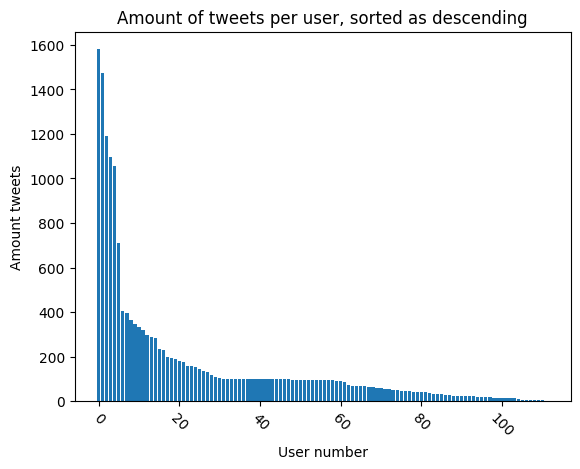
\includegraphics[scale=0.6]{figures/amount_tweets_per_user}
        \caption{Amount of tweets per user}
        \label{fig:amount-tweets-user}
    \end{figure}

    Loglikelihood ratios where compared to estimate the most likely fit.
    We can see from the table~\ref{tab:powerlaw} the most likely fit might be Truncated Power Law.
    Comparison between different distributions are pointing that lognormal or truncated power law are the most likely, where truncated power law is significantly stronger fit (p $>$ 0.05).
    Usually this means we might have too many data entries and the rest of the data "fall-off" from the power law or simply not enough data.
    We might be able to analyse tails bit better, but it is left out of the scope in this assignment.

    \begin{figure}
        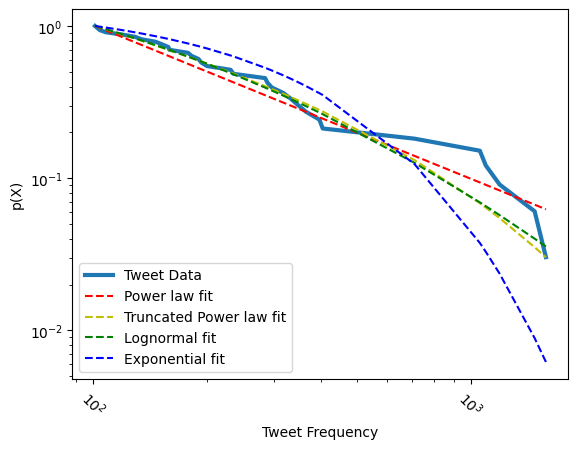
\includegraphics[scale=0.5]{figures/amount_tweets_powerlaw}
        \caption{Distribution candidates for amount of tweets per user}
        \label{fig:amount-tweets-powerlaw}
    \end{figure}

    Data was further sorted for top 10 users by mentions, retweets and hashtag usages and plotted by Matplotlib.
    Results are shown in the figure~\ref{fig:amount-mentions-user},~\ref{fig:amount-retweets-user}, and~\ref{fig:amount-hashtags-user}.
    Usernames are partially shortened to not make them totally public.

    These three figures show that similar usernames are appearing on all three categories, but mostly in different order.
    This might be partially explained with the power law, as minority of the user amount are mostly responsible from the tweets,
    and with enough content diversity of the tweets, they can reach top position on multiple categories.
    Based on this, these users are effectively using properties of Twitter platform to connect to other users, potentially gaining more visibility.
    These users are mainly responsible on distributing messages and sharing other messages, giving visibility with hashtags.


    \begin{figure}
        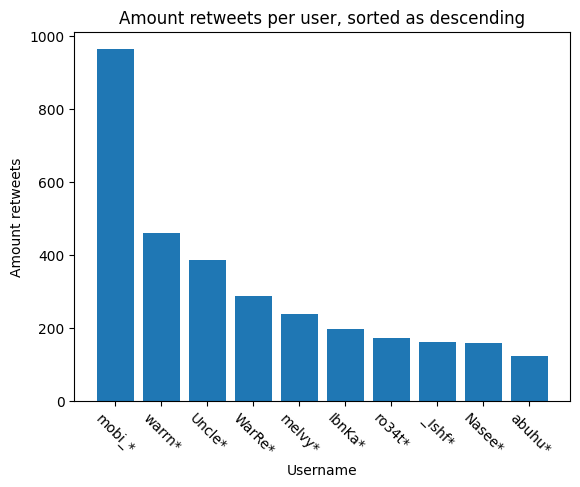
\includegraphics[scale=0.6]{figures/amount_retweets_user}
        \caption{Top10 users by retweeting.}
        \label{fig:amount-retweets-user}
    \end{figure}

    \begin{figure}
        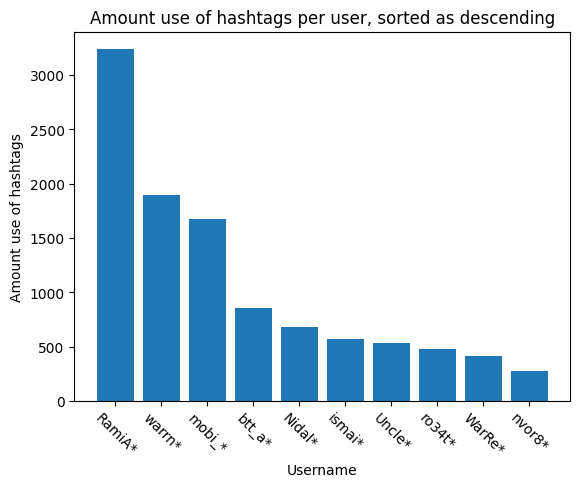
\includegraphics[scale=0.6]{figures/amount_hashtags_user}
        \caption{Top10 users by usage of hashtags.}
        \label{fig:amount-hashtags-user}
    \end{figure}

    \begin{figure}
        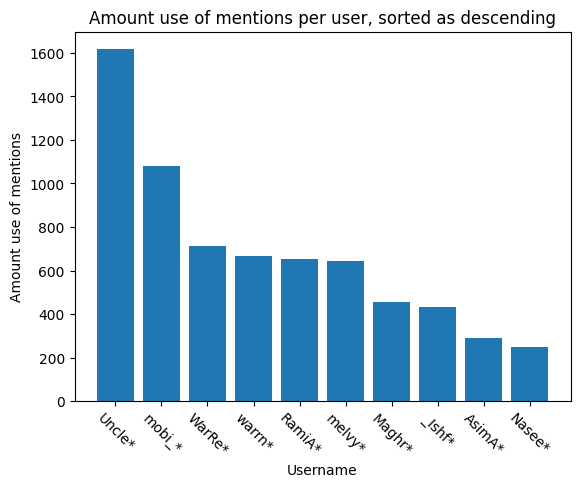
\includegraphics[scale=0.6]{figures/amount_mentions_user}
        \caption{Top10 users by usage of mentions.}
        \label{fig:amount-mentions-user}
    \end{figure}
    \begin{table}
        \begin{tabular}{ |c|c|c|c|}
            \hline
            Distribution 1 & Distribution 2      & R     & \textit{p} \\
            \hline
            Power Law      & Lognormal           & -0.96 & 0.34       \\
            \hline
            Power Law      & Exponential         & 0.83  & 0.40       \\
            \hline
            Exponential    & Lognormal           & -1.65 & 0.10       \\
            \hline
            Power Law      & Truncated Power Law & -1.34 & 0.10       \\
            \hline
            Lognormal      & Truncated Power Law & -0.36 & 0.27       \\
            \hline
        \end{tabular}
        \caption{Loglikelihood rations of the different distributions}
        \label{tab:powerlaw}
    \end{table}

    \subsection{Sentiment analysis}
    Sentiment analysis was applied for whole tweet data and separately for tweets of previously calculated top10 users by different categories.

    In the figure \ref{fig:sentiment-ternary-all} we can see ternary plot of sentiment analysis among all tweets.
    Distribution isn't totally clear, as there are many values with zero negative or positive weight, which leads points to be on the border of the ternary.

    On a quick glance it seems that tweets are more weighted on negative side in general.
    After taking exact numbers, negative seems to have slight majority, and positive is in clear minority.

    \begin{itemize}
        \item Amount of NEGATIVE values: 6948
        \item Amount of NEUTRAL values: 6657
        \item Amount of POSITIVE values: 3805
    \end{itemize}

    It implies that content of tweets is siding more on negative/neutral side than neutral/positive side in general.

    In figure \ref{fig:sentiment-ternary-user-hashtag} we can see ternary plot, where tweets are limited to top 10 users by usage of hashtags.
    In figure \ref{fig:sentiment-ternary-user-mention} ternary plot is constructed by usage of mentions of top 10 users.
    Finally in the figure \ref{fig:sentiment-ternary-user-retweet} ternary plot is created by the use of retweets.

    It is difficult to see drastic differences by the eye on ternary plots. The most significantly it seems that users with the most use
    of hashtags, sentiment value seems to be mostly negative.

    \begin{figure}
        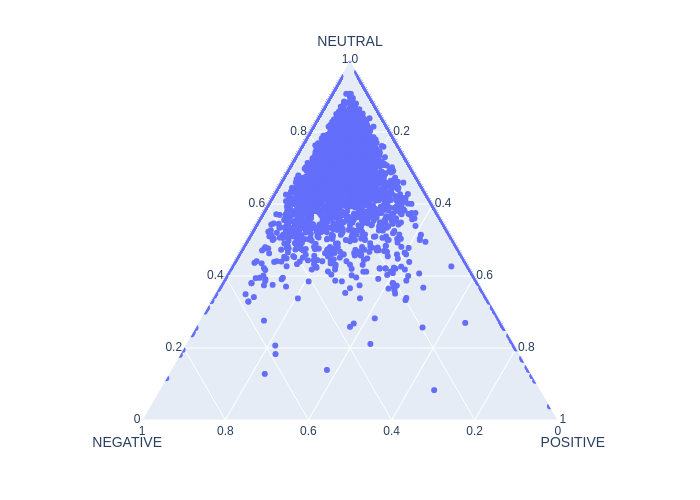
\includegraphics[scale=0.4]{figures/sentiment_ternary_all}
        \caption{Ternary plot of sentiment analysis of all tweets.}
        \label{fig:sentiment-ternary-all}
    \end{figure}

    \begin{figure}
        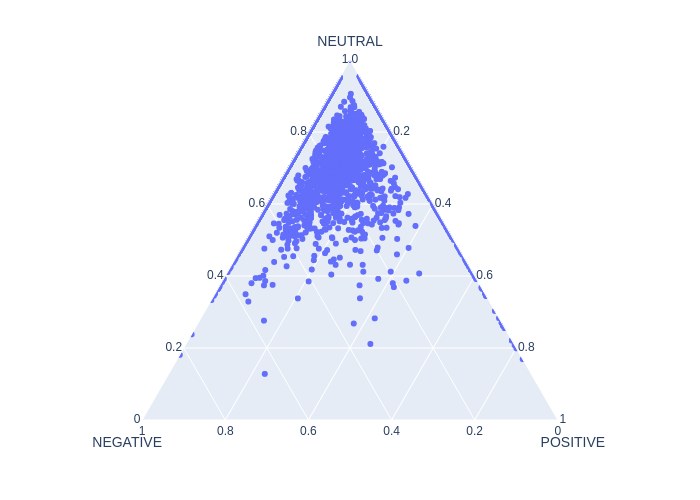
\includegraphics[scale=0.4]{figures/sentiment_ternary_amount_hashtags}
        \caption{Ternary plot of tweets combined of top10 users by usage of hashtags }
        \label{fig:sentiment-ternary-user-hashtag}
    \end{figure}

    \begin{figure}
        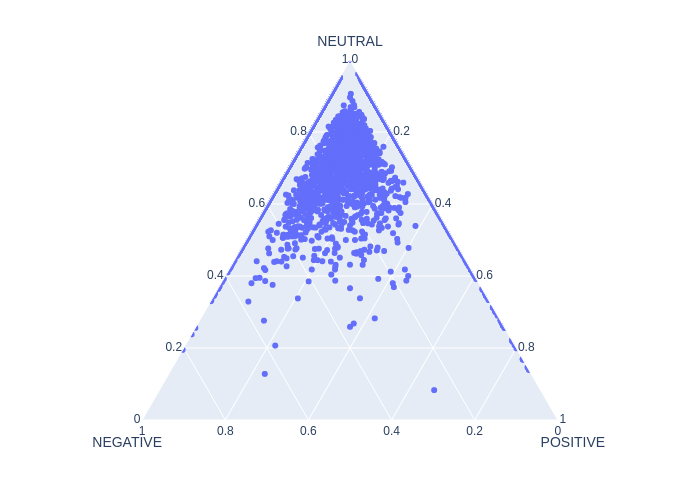
\includegraphics[scale=0.4]{figures/sentiment_ternary_amount_mentions}
        \caption{Ternary plot of tweets combined of top10 users by usage of mentions }
        \label{fig:sentiment-ternary-user-mention}
    \end{figure}

    \begin{figure}
        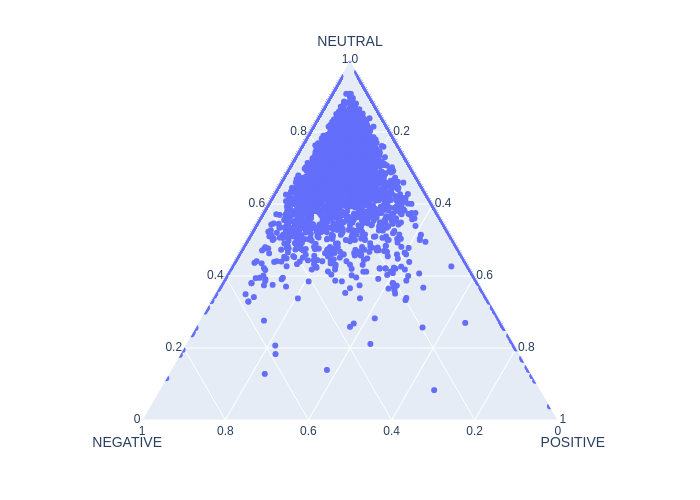
\includegraphics[scale=0.4]{figures/sentiment_ternary_all}
        \caption{Ternary plot of tweets combined of top10 users by retweeting }
        \label{fig:sentiment-ternary-user-retweet}
    \end{figure}


    \begin{table*}[ht]
        \begin{tabular} { | c | c | c | c | c | c | c | c | c | }
            \hline
            k & Nodes \# & Edges \# & Largest component & Diameter & Avg. Clustering Coef. & Avg. Degree
            & Avg. Closeness
            & Avg. Betweenness
            \\
            \hline
            1  & 2347 & 8215 & 1877 & 9  & 0.59 & 7.0  & 0.2  & 0.0 \\
            \hline
            2  & 2347 & 2149 & 591  & 9  & 0.16 & 1.83 & 0.02 & 0.0 \\
            \hline
            3  & 2347 & 1094 & 339  & 11 & 0.07 & 0.93 & 0.01 & 0.0 \\
            \hline
            4  & 2347 & 753  & 218  & 6  & 0.05 & 0.64 & 0.0  & 0.0 \\
            \hline
            5  & 2347 & 561  & 177  & 6  & 0.05 & 0.48 & 0.0  & 0.0 \\
            \hline
            10 & 2347 & 249  & 89   & 5  & 0.02 & 0.21 & 0.0  & 0.0 \\
            \hline
            15 & 2347 & 156  & 59   & 4  & 0.01 & 0.13 & 0.0  & 0.0 \\
            \hline

        \end{tabular}
        \caption {Core measurements of hashtag graph by minimal hashtag pair occurrences (k)}
        \label {tab:graphstats-by-k}
    \end{table*}

    \begin{table*}[ht]
        \begin{tabular} { | c | c | c | c | c | c | c | c | c | }
            \hline
            k & Nodes \# & Edges \# & Largest component & Diameter & Avg. Clustering Coef. & Avg. Degree
            & Avg. Closeness
            & Avg. Betweenness
            \\
            \hline
            1  & 2078 & 8215 & 1877 & 9  & 0.66 & 7.91 & 0.26 & 0.0  \\
            \hline
            2  & 653  & 2149 & 591  & 9  & 0.57 & 6.58 & 0.28 & 0.0  \\
            \hline
            3  & 374  & 1094 & 339  & 11 & 0.46 & 5.85 & 0.28 & 0.0  \\
            \hline
            4  & 244  & 753  & 218  & 6  & 0.51 & 6.17 & 0.31 & 0.01 \\
            \hline
            5  & 192  & 561  & 177  & 6  & 0.55 & 5.84 & 0.33 & 0.01 \\
            \hline
            10 & 96   & 249  & 89   & 5  & 0.51 & 5.19 & 0.37 & 0.01 \\
            \hline
            15 & 64   & 156  & 59   & 4  & 0.55 & 4.88 & 0.39 & 0.02 \\
            \hline

        \end{tabular}
        \caption {Core measurements of hashtag graph by minimal hashtag pair occurrences (k), removing nodes without connections}
        \label {tab:graphstats-by-k-no-connect}
    \end{table*}

    \subsection{Hashtag Network Analysis}

    Hashtag network was build successfully with NetworkX.
    To get initial visual view, we can take a glance on figure \ref{fig:graph-general} and figure \ref{fig:graph-general-zoomed} on Appendixes.
    There is one giant community.
    This graph was created with $k$ = 0; e.g. all nodes are included.
    We wanted also to examine graph by the amount of hashtag pair occurrences $k$, which limits only those hashtags pairs into the network
    which are used at least $k$ times.
    The core properties can be seen in the tables \ref{tab:graphstats-by-k} and \ref{tab:graphstats-by-k-no-connect}.
    Only difference with these two tables are, that table \ref{tab:graphstats-by-k-no-connect} has nodes removed which are not
    fulfilling the $k$ requirement.
    Visual graph with reduced graph ($k$ = 2 was selected), we can see the core structure bit better in the figure \ref{fig:graph-general-k2}.

    \begin{figure}
        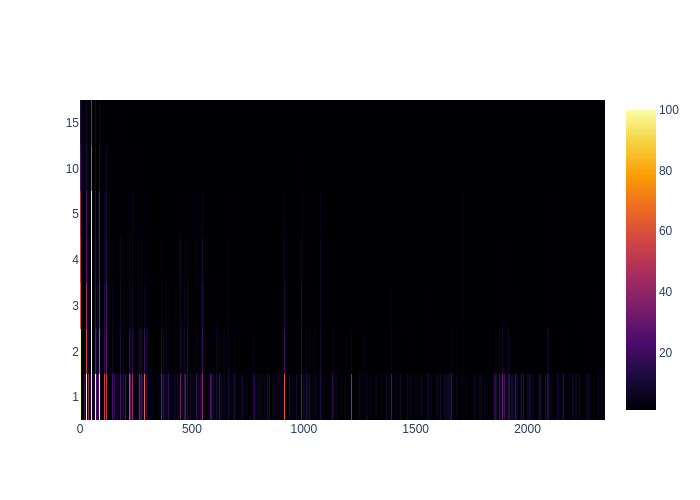
\includegraphics[scale=0.32]{figures/hashtag_heatmap_by_k}
        \caption{Heatmap of the hashtag graph, with $k$ values 1, 2, 3, 4, 5, 10, 15}
        \label{fig:hashtag-heatmap}
    \end{figure}

    There are around 4x amount of edges compared to nodes, hence the network has many connections, when looking at without $k$ limitations.
    All nodes are not connected and diameter was estimated based on the biggest component.
    It was expected that network will not be totally connected - some specific hashtag might appear only alone in the tweet.

    The effect of $k$ requirement can be seen clearly.
    Some hashtag pairs are used very often with other hashtags as we can find plenty of nodes even with $k$ = 15,
    and they are creating close communities as closeness and inbetweenness values are increasing.
    For reference, list of ranked hashtags with $k$ = 15 can be found from the table \ref{tab:hashtag-ranks-k-15} in Appendixes.
    Degree centrality and clustering coefficient are not changing significantly, which implies that on average hashtags are used quite "equally" with other hashtags.
    Plotted heatmap is pointing also the importance of some hashtags over others in the figure \ref{fig:hashtag-heatmap}.
    Maximum value in the heatmap is limited into 100, because few hashtag occurrences were significantly more frequent (400+) than others, making heatmap hard to observe.


    For further ranking these connections, PageRank distribution has also been calculated and can be seen on the figure \ref{fig:pagerank}.
    Based on the figure, we can deduce that small portion of hashtags has significantly higher rank value that most of them.
    Out of the curiosity, top 10 hashtag names based on PageRank are listed in the table \ref{fig:sentiment-ternary-all}.
    When comparing to custom generated table~\ref{tab:hashtag-ranks-k-15}, we can find similar hashtags from the top10.
    Note, that names are normalized to be lowercase, since they are case-insensitive when construction networks on Twitter platform behind the scenes.

    Histogram of LCC can be seen in the figure \ref{fig:lcc}.
    As the total amount of nodes (unique hashtags) were 2347 in initial graph, we can see that clear majority of them has either LCC value close to zero (600+) or 1 (more than 1000), meaning
    they have barely connections or they are almost fully connected, being "complete graph".

%    If we combine this information to all what we found before, we can say that the network has some core hashtags, which are used often with
%    other hashtags. Many different users are using these same hashtags, probably in strict group.
%    Then there are some "random" cases when these same hashtags are used, but less with other hashtags.

    \begin{table}
        \begin{tabular}{ |c|c|}
            \hline
            Rank # & Hashtag         \\
            \hline
            1      & isis            \\
            \hline
            2      & islamicstate    \\
            \hline
            3      & syria           \\
            \hline
            4      & is              \\
            \hline
            5      & breaking        \\
            \hline
            6      & amaqagency      \\
            \hline
            7      & iraq            \\
            \hline
            8      & caliphate\_news \\
            \hline
            9      & aleppo          \\
            \hline
            10     & assad           \\
            \hline
        \end{tabular}
        \caption{Top10 hashtags by PageRank}
        \label{tab:hashtag-names}
    \end{table}



    \begin{figure}
        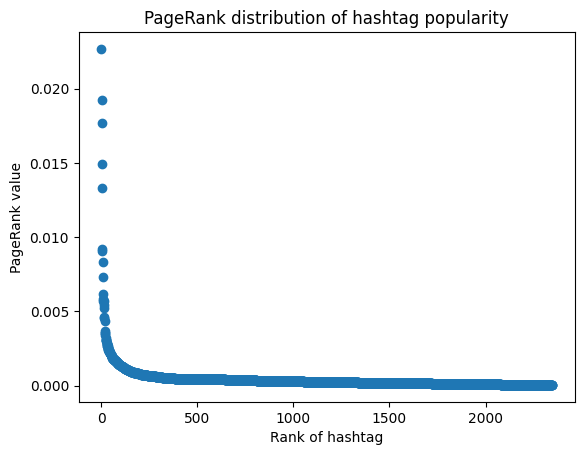
\includegraphics[scale=0.6]{figures/pagerank_distribution}
        \caption{PageRank of different hashtags.}
        \label{fig:pagerank}
    \end{figure}

    \begin{figure}
        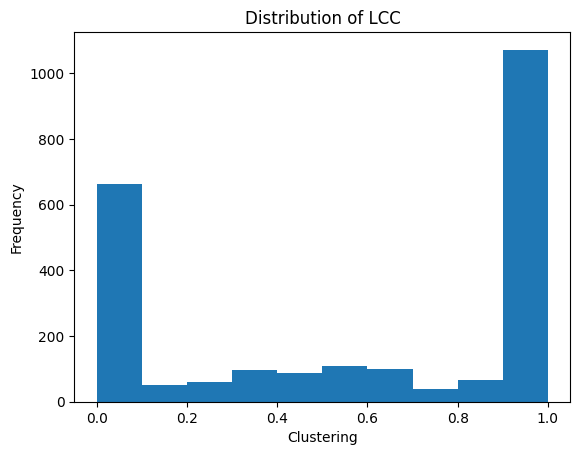
\includegraphics[scale=0.6]{figures/lcc_distribution}
        \caption{Local Clustering Coefficient distribution}
        \label{fig:lcc}
    \end{figure}

    To get more information about underlying communities inside network, Girwan-Newmann algorithm was used.
    Based on the initial visual graphs, iteration value of 10 was initially selected as depth to get communities.
    It looked a good candidate to limit communities to the biggest ones inside the first giant community.
    However, it appeared to be ineffective, and reduced the giant community only into the size of 1654 nodes, when the initial size was 1877.

    At this point, we had top 5 communities with following sizes:

    \begin{enumerate}
        \item 1654
        \item 145
        \item 33
        \item 16
        \item 8
    \end{enumerate}

    The first community is still too big to estimate content based on the used hashtags.
    Due to time concerns, no more details are extracted in this case.
    The second community is interesting in terms of size  - and based on the hashtag contents, it seems to be fully using foreign language hashtags,
    potentially in arabic.
    It is potentially a community which does not use English as the majority of the tweets are using.
    Third community seems to be using foreign language as well.
    Fourth community seems to be related on cyber topic, containing hashtags for example of 'cyberjihad', 'cybernews', 'hacked', 'status', 'ucc', 'website'.
    Fifth community seems to be related on the Islam religion, with limited amount of hashtags is is harder to limit more.


    \section{Conclusion and Perspectives}\label{sec:conclusion-and-perspectives}

    Network from over 17~000 tweets was constructed by using identified connections with hashtags.
    So far results have been interpreted from statistical point of view, generalizing results for Twitter platform.
    Based on the results, we could identify potential core accounts behind pro-ISIS fanboys on distributing messages.
    The way how tweets are distributed (e.g. Tweet frequency per user seems to follow truncated power law)
    tells that only a limited amount of users are mostly responsible about them.
    Similar observations have been identified in other studies such as "Pro-ISIS fanboys network analysis and attack detection through Twitter data"\cite{8078846} which used same dataset.
    In the study, selected amount of users were identified to be with the most influence, being similar usernames than in this study.

    These core accounts are using Twitter very efficiently; they use limited set of hashtags (such as ISIS, Iraq, Syria, Breaking, Aleppo) with other hashtags, on repeating matter.
    Use of multiple hashtags with preserving core hashtags supports this.
    Different topics are efficiently connected together, possibly making core hashtags "trending" on the platform.
    Hashtags are potentially granting a way to broadcast topics while avoiding ban from the platform when compared to other places (e.g. public forum)

    Similar accounts appear to be top 10 on use of mentions, retweeting and using of hashtags.
    Based on sentiment analysis, the tweet contents appear to be mostly negative, which is not surprise, as data is coming from terrorism organization fanboys.
    Negativity seems to be more significant when viewed from the point of hashtags, retweets or mentions.
    This could imply negative contents to finally attract more attention.

    Only by removing top 10 accounts in terms of tweets, we could potentially decrease the underlying communities significantly in this network.

    Girvan-Newman algorith was used to detect underlying communities.
    Due to time constraints, only brief look for top level communities were looked.
    It was able to detect communities using foreign language, handling cyber security related content and purely Islam religion related.
    We can speculate, that these are outside the main message, what this specific network is handling, and that is also the reason why they were firstly removed from the whole network.

    We can link the dataset directly to ISIS based on the most influencing node (hashtag) names in the network.

    Overall, graph study seems to be efficient way to study networks appearing in the Twitter platform.
    ISIS is using Twitter really efficiently to distribute their message.


    \bibliographystyle{./IEEEtran}
    \bibliography{./IEEEabrv,./references}
%\vspace{12pt}

    \newpage
    \section*{Appendix}

    \begin{figure*}
        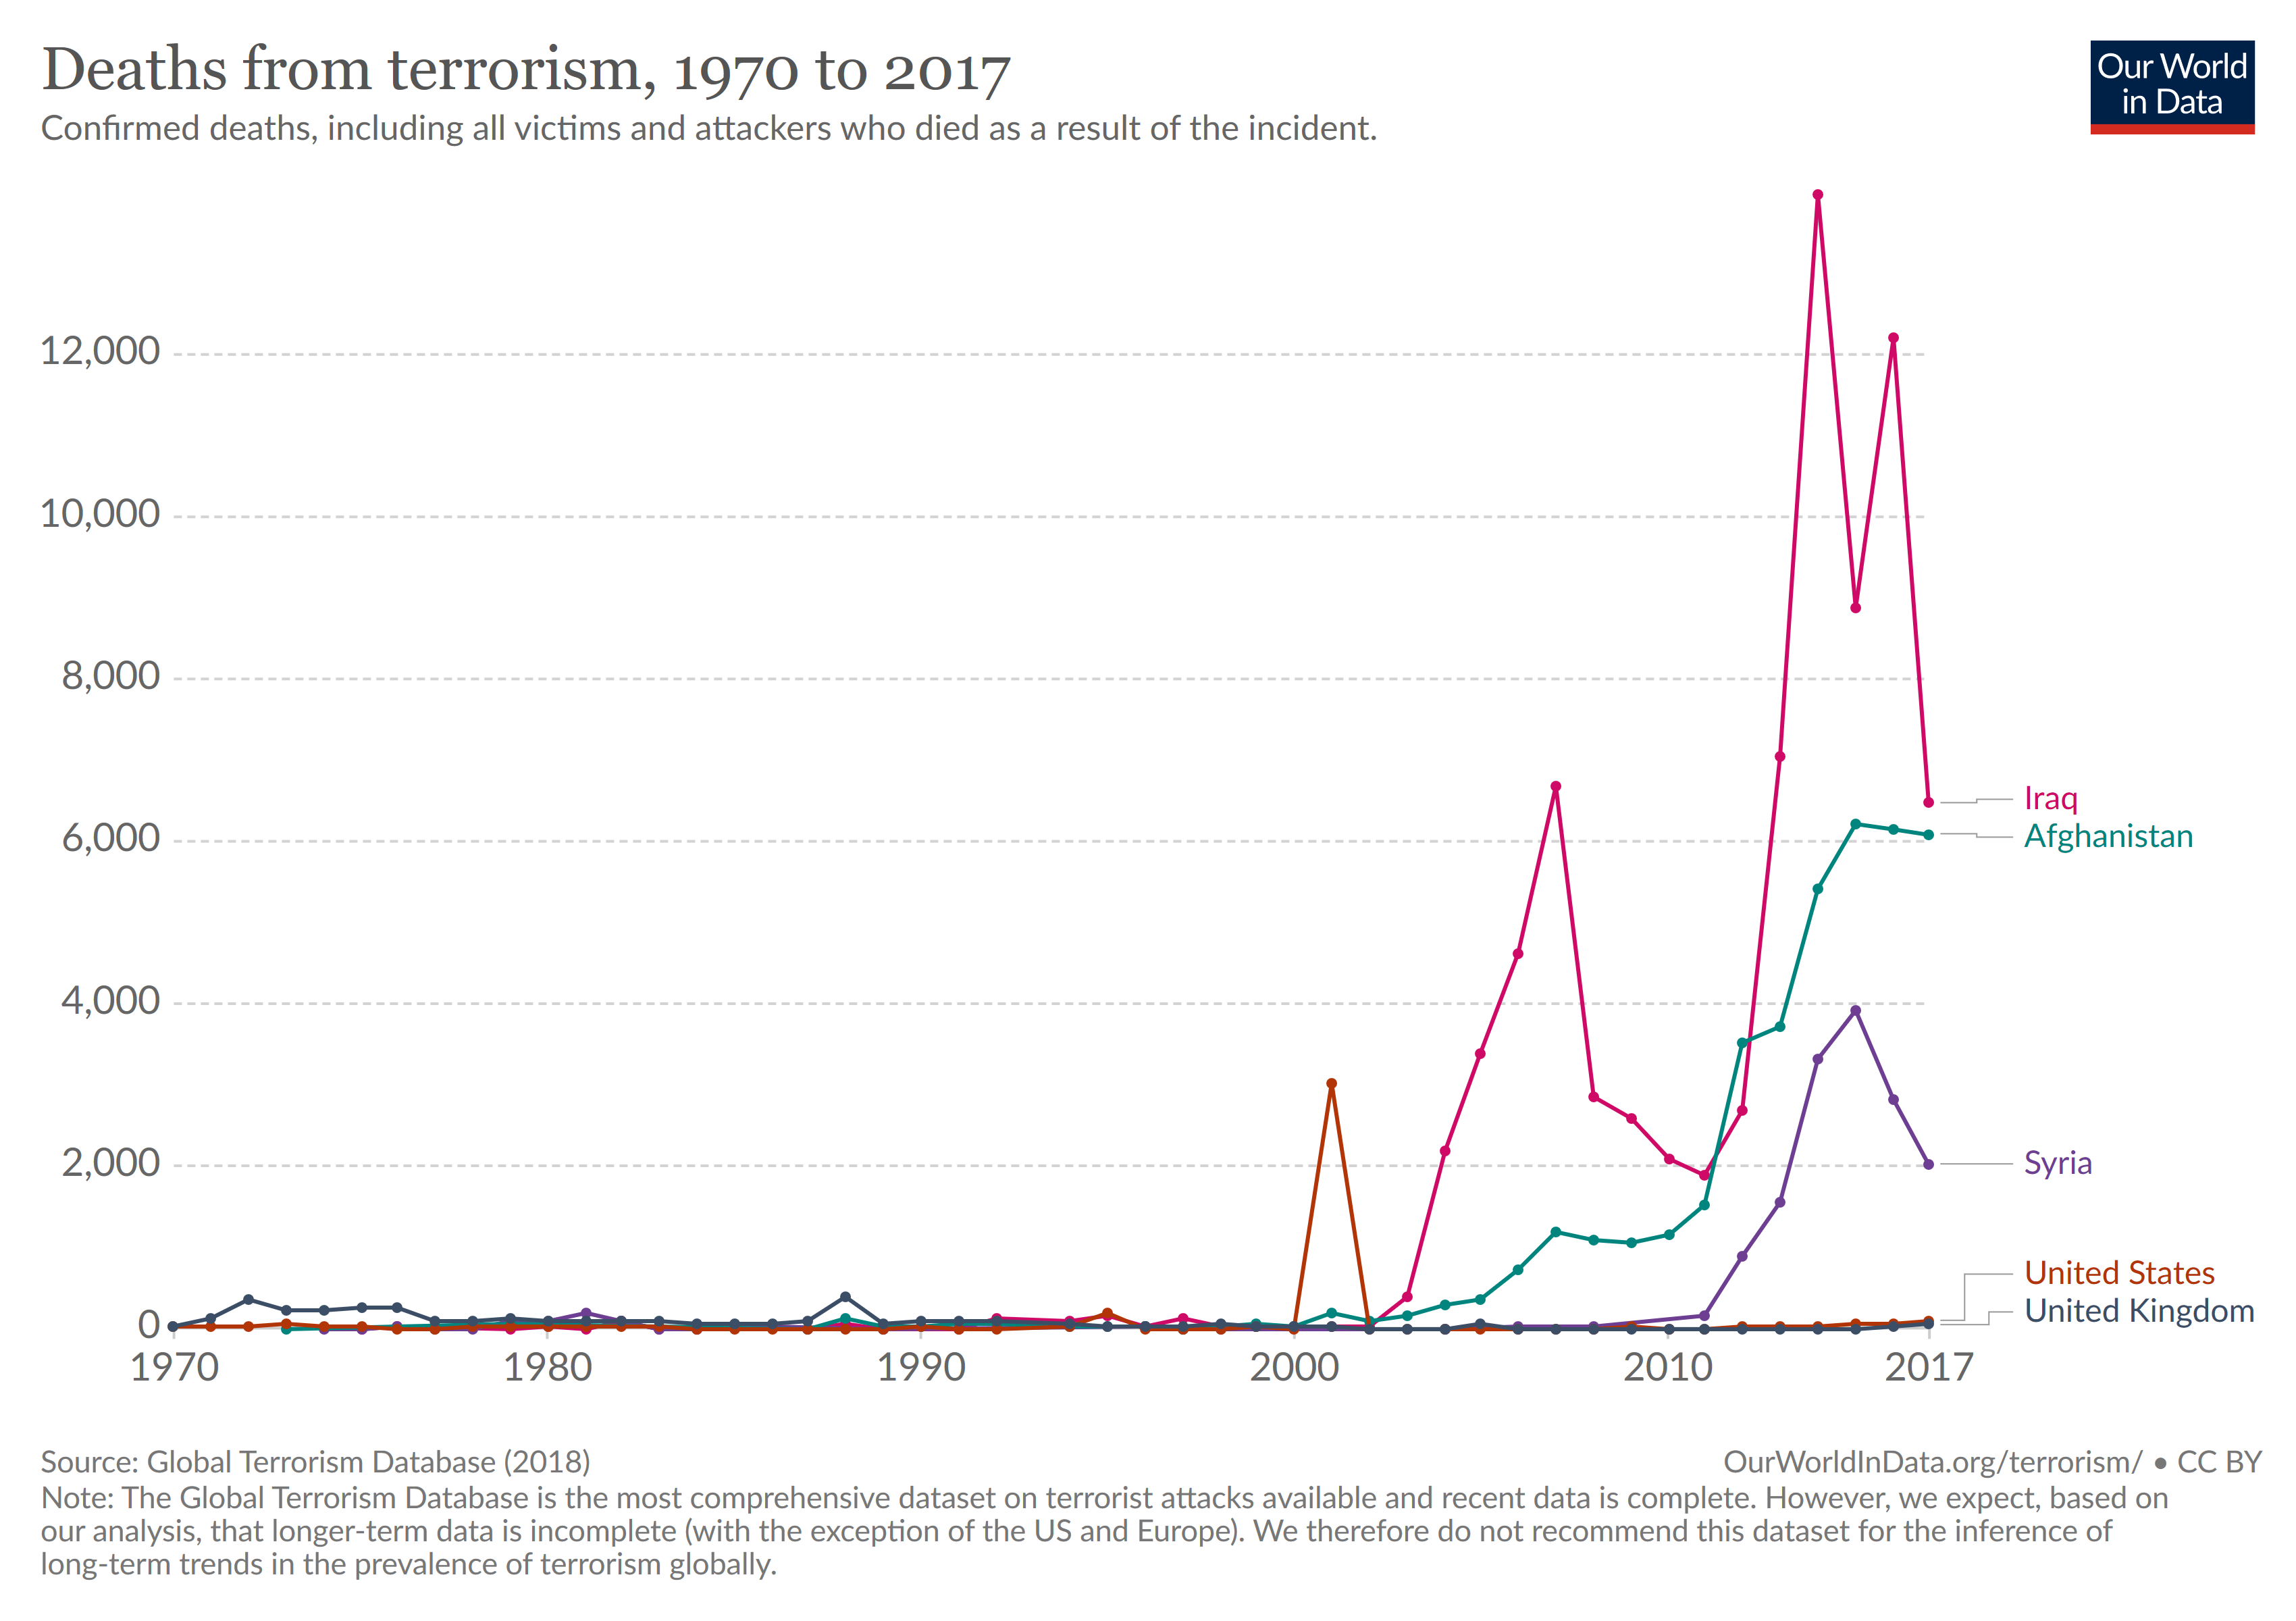
\includegraphics[scale=0.15]{figures/fatalities-from-terrorism}
        \caption{Deaths from terrorism, 1970--2017.}
        \label{fig:appendix_terrorism_deaths}
    \end{figure*}\label{subsec:data-verification-after-some-pre-processing-methods}

    \begin{figure*}
        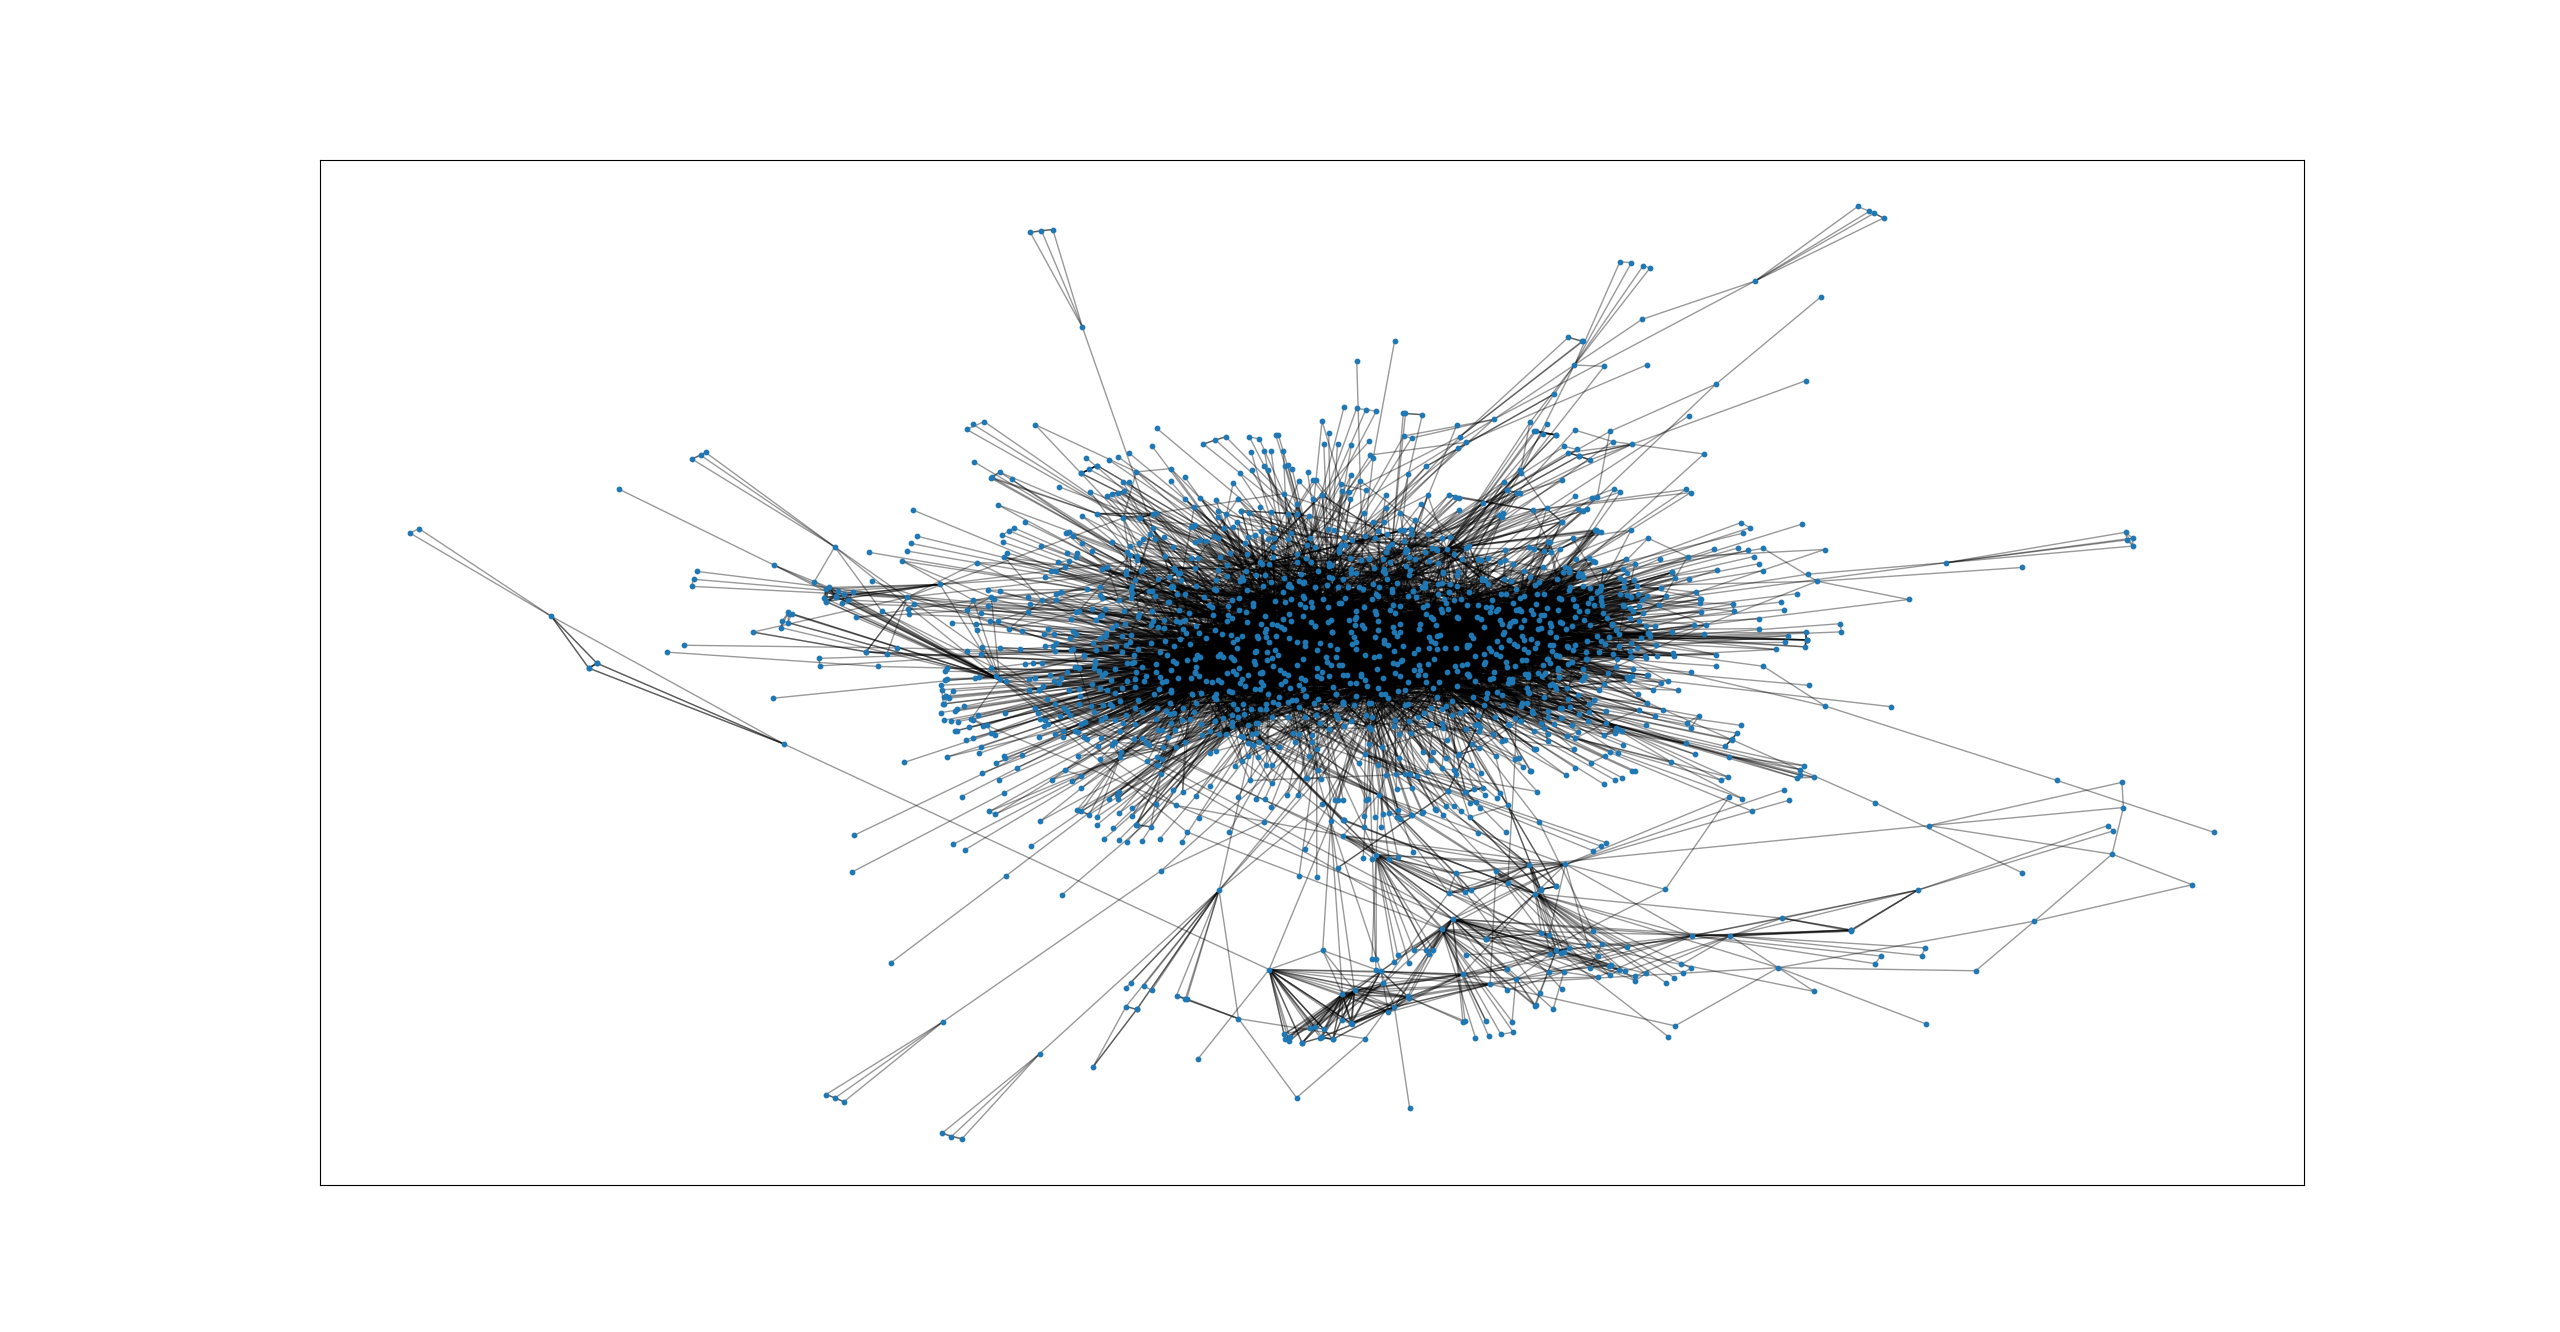
\includegraphics[scale=0.32]{figures/general_graph}
        \caption{General view of the hashtag graph. One giant commumity.}
        \label{fig:graph-general}
    \end{figure*}

    \begin{figure*}
        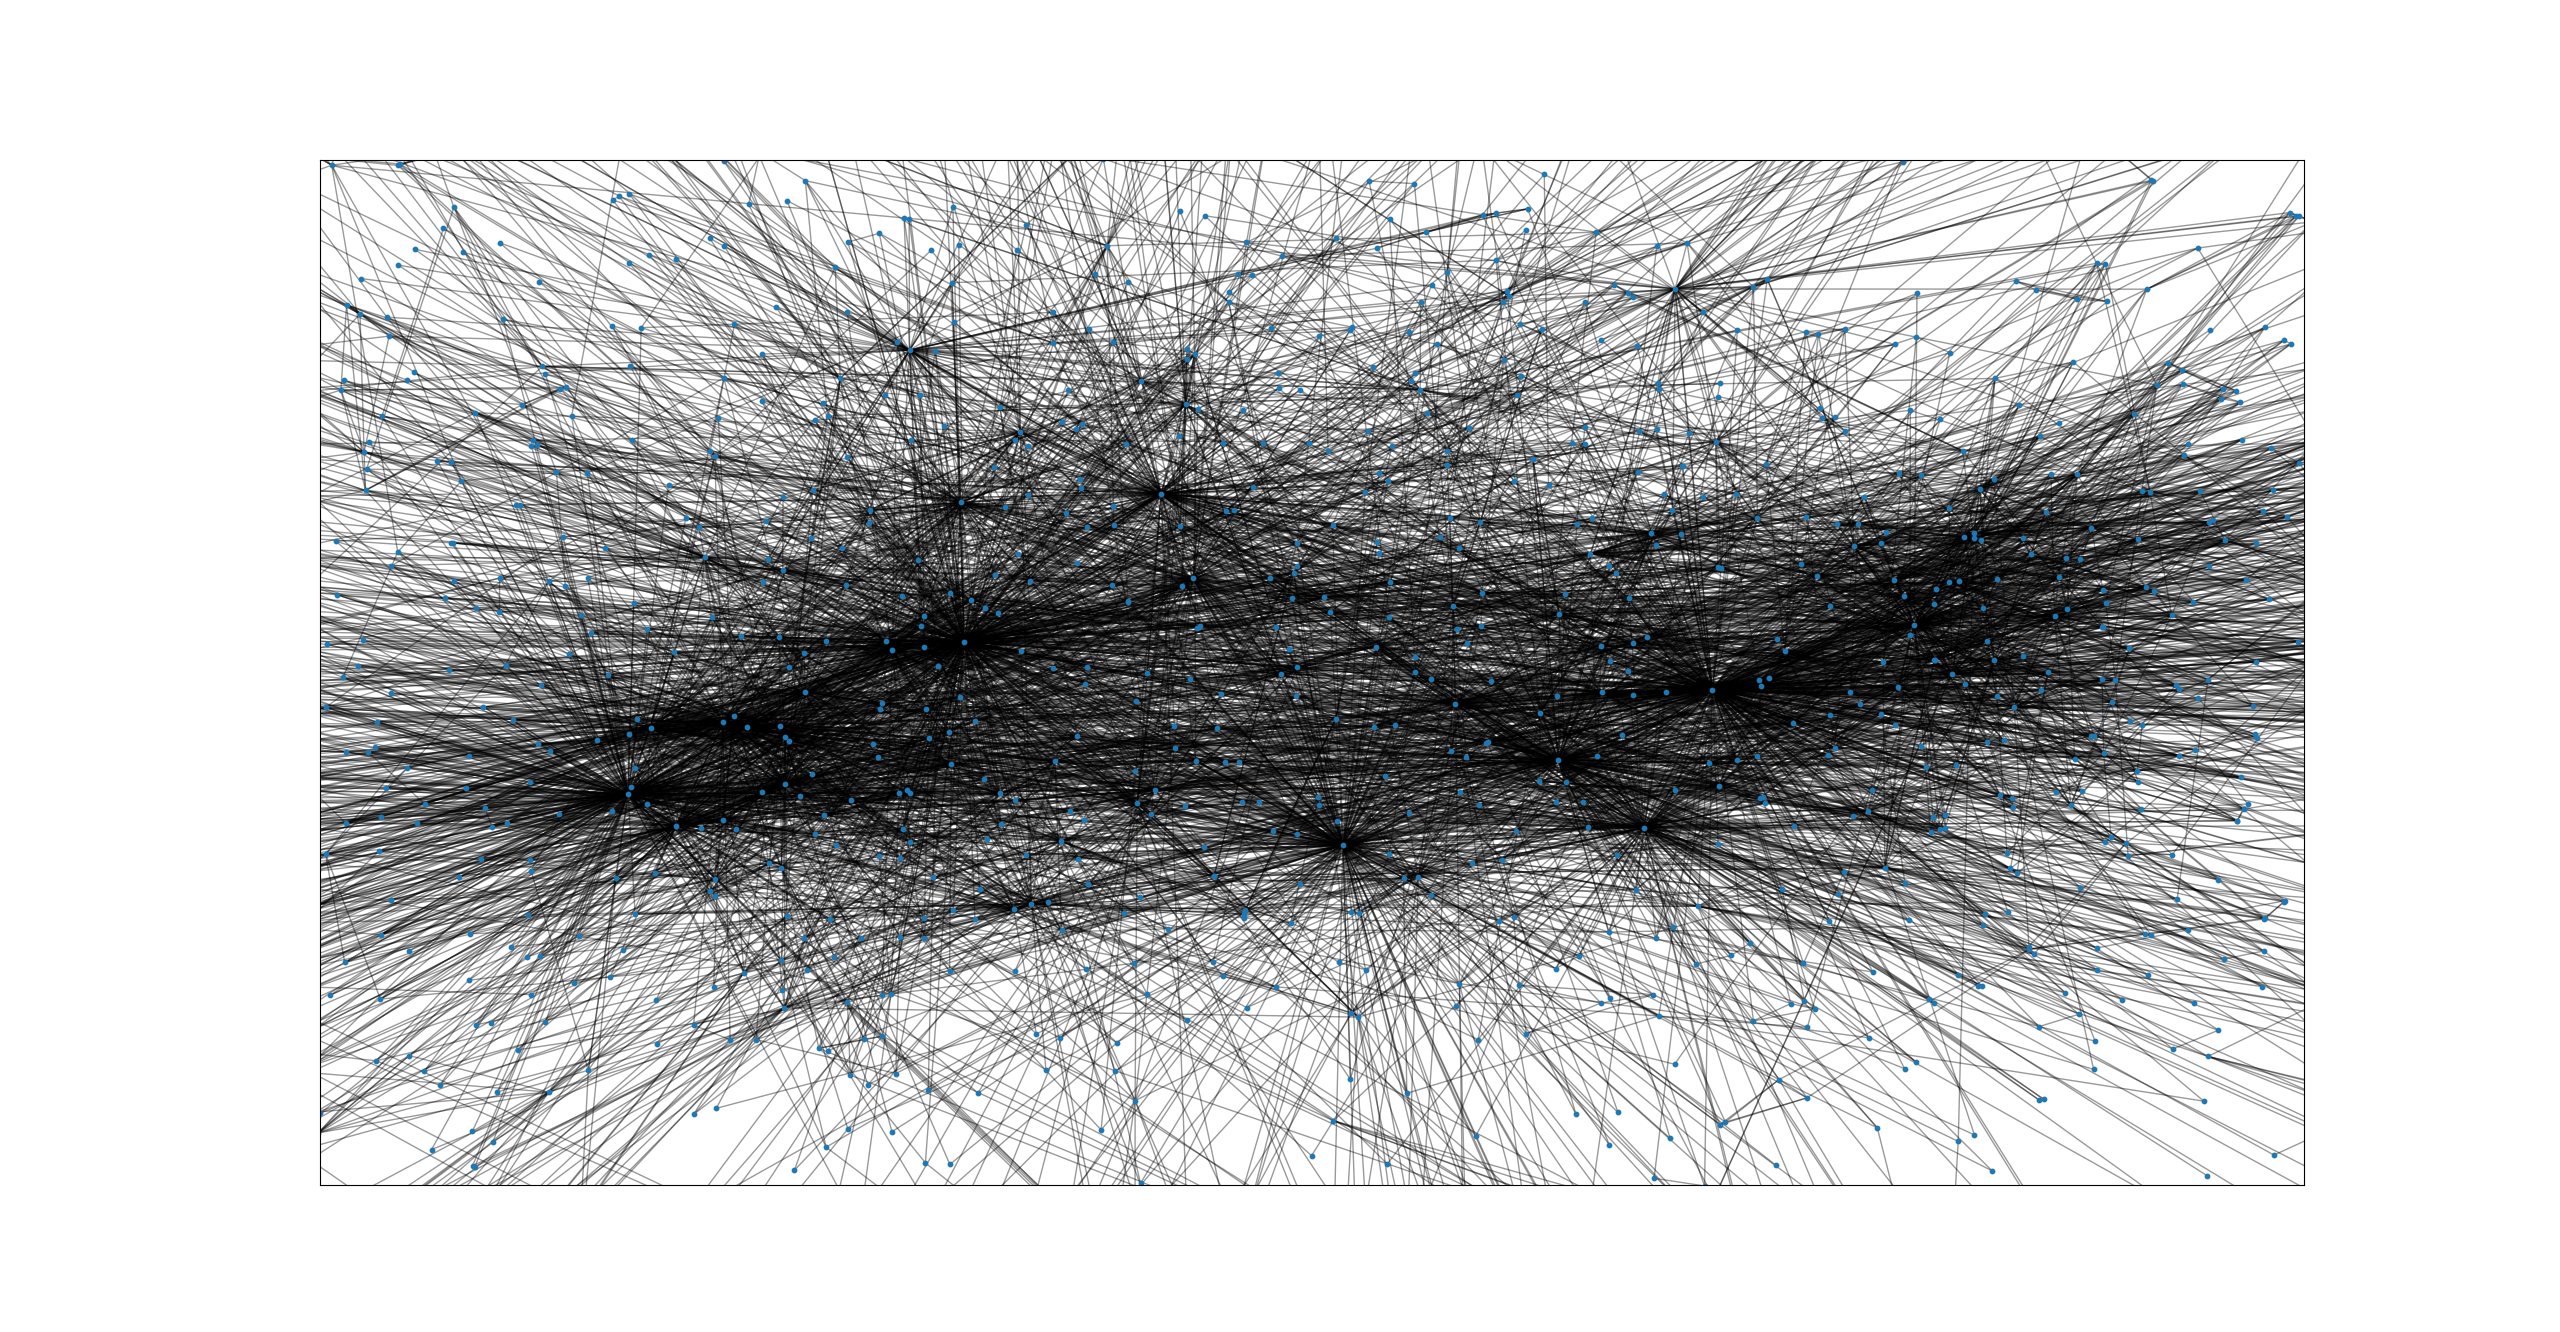
\includegraphics[scale=0.32]{figures/general_graph_zoomed}
        \caption{Zoomed view to the giant community reveals more communities.}
        \label{fig:graph-general-zoomed}
    \end{figure*}
    \begin{figure*}
        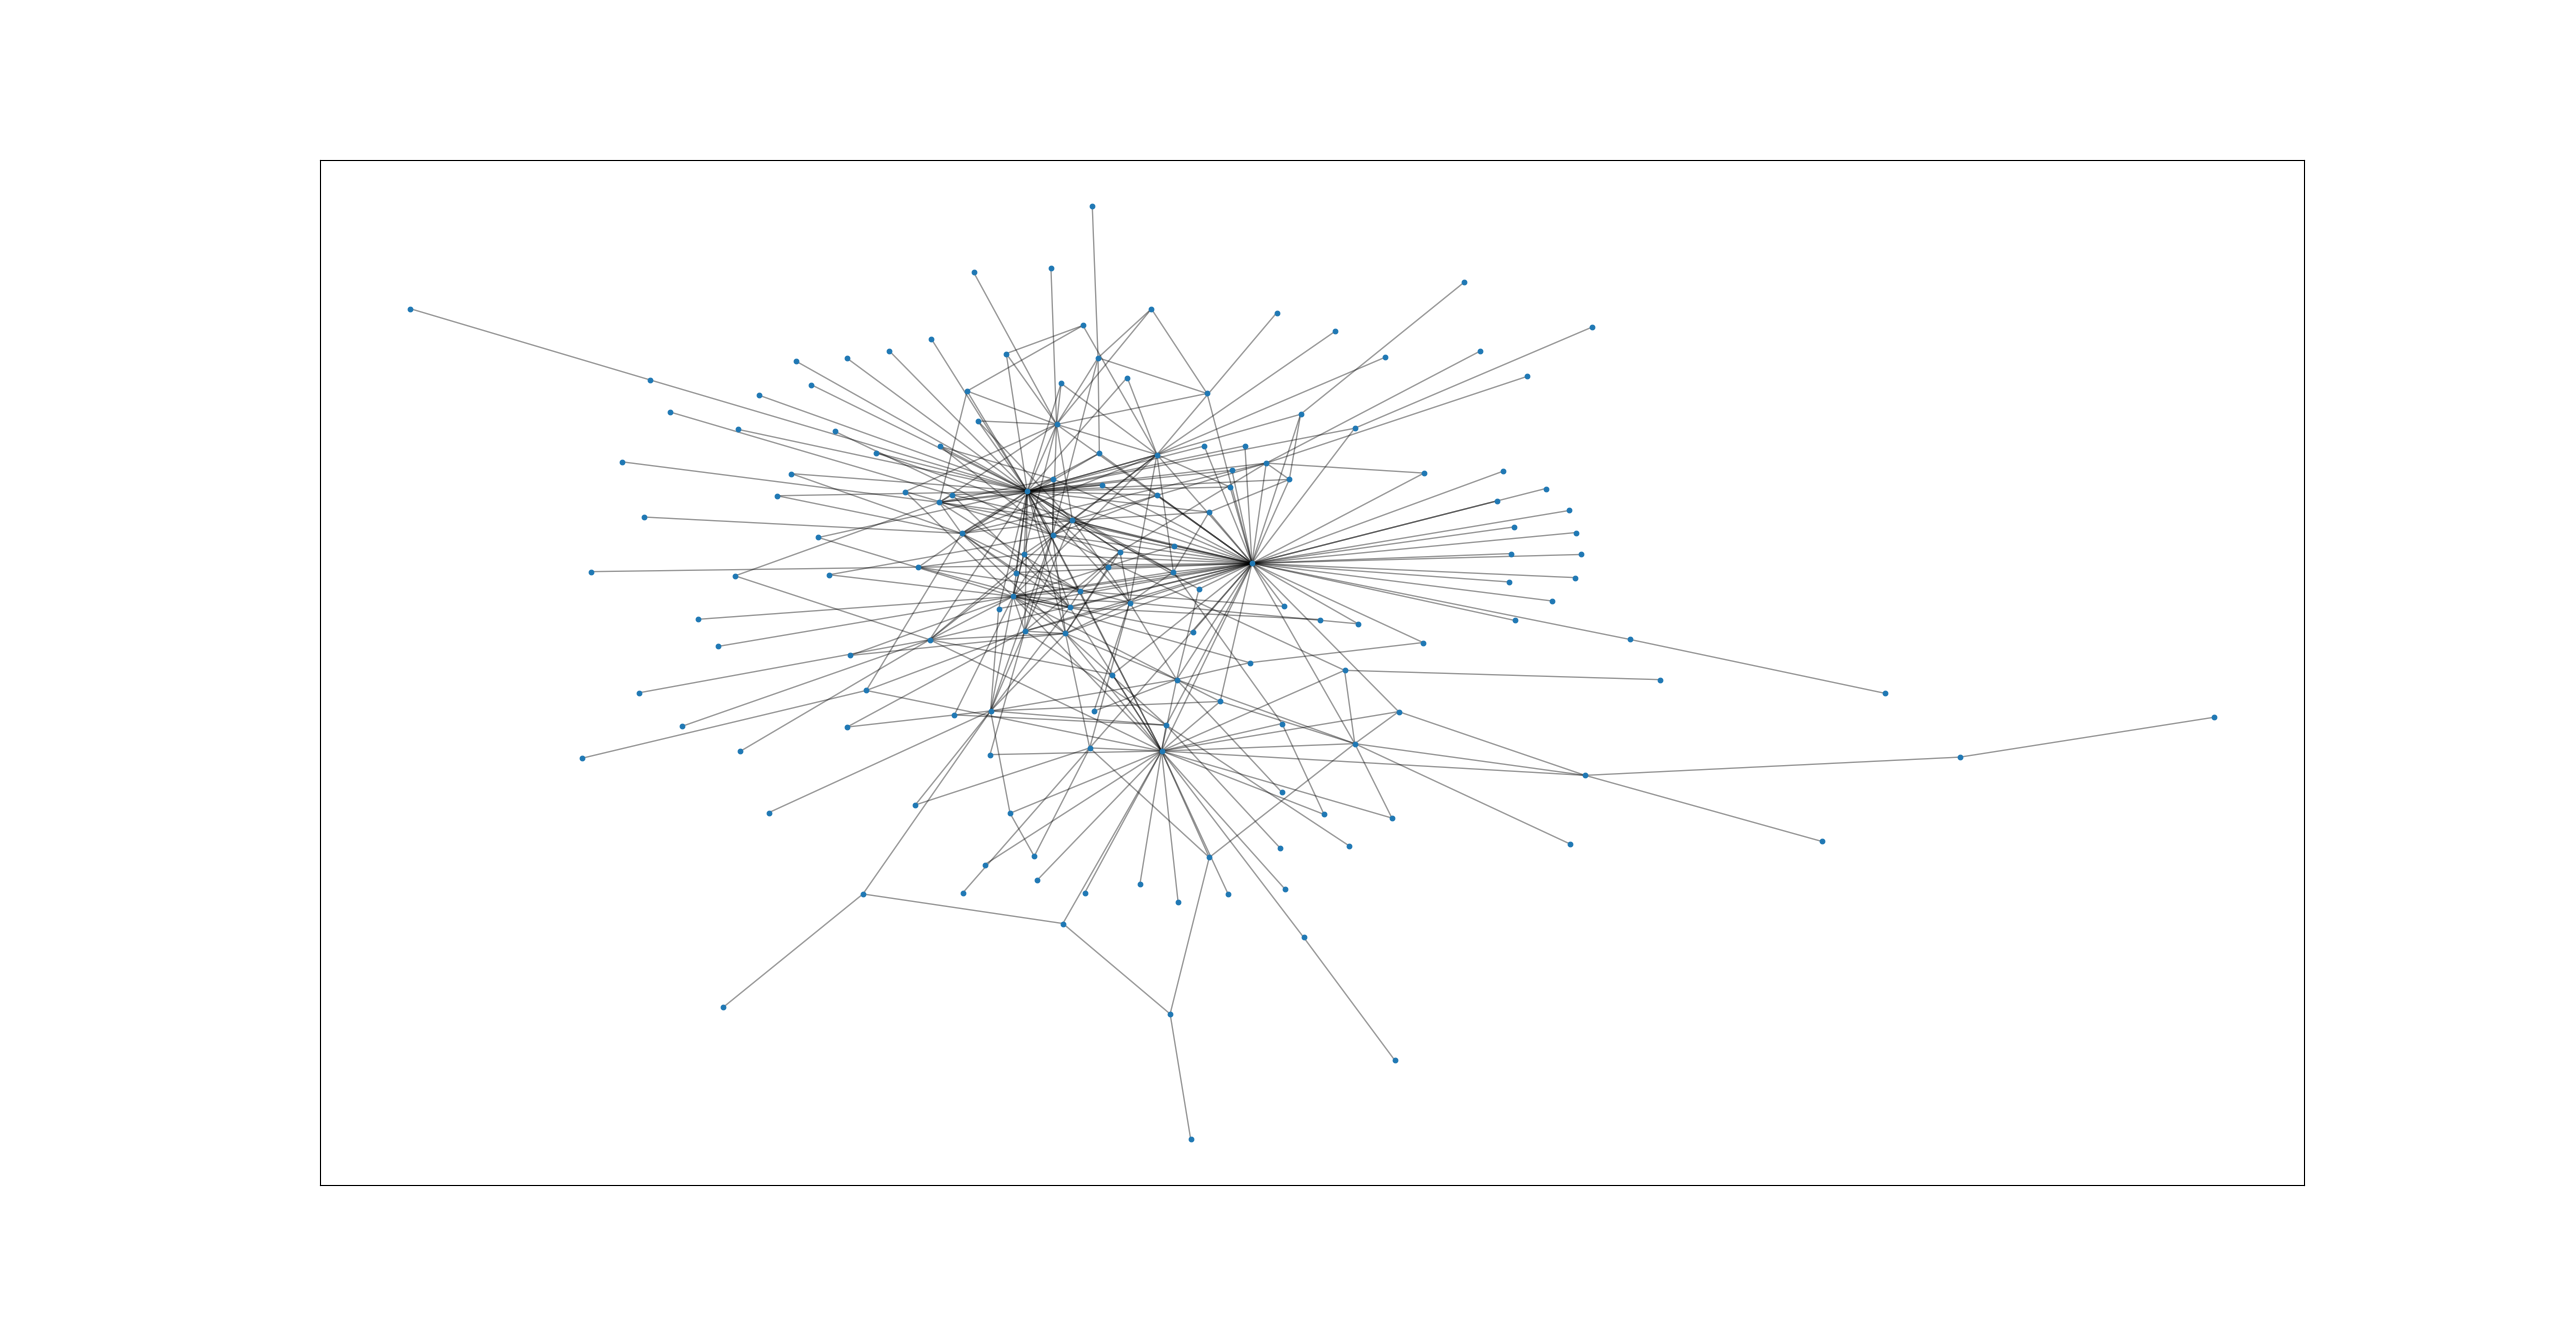
\includegraphics[scale=0.32]{figures/general_graph_k_2}
        \caption{General view of the hashtag graph. $k$ = 2}
        \label{fig:graph-general-k2}
    \end{figure*}

    \begin{table}[ht]
        \begin{tabular} { | c | c | }
            \hline
            Rank & Hashtag         \\
            \hline
            1    & isis            \\
            \hline
            2    & syria           \\
            \hline
            3    & iraq            \\
            \hline
            4    & is              \\
            \hline
            5    & aleppo          \\
            \hline
            6    & islamicstate    \\
            \hline
            7    & breakingnews    \\
            \hline
            8    & assad           \\
            \hline
            9    & ypg             \\
            \hline
            10   & turkey          \\
            \hline
            11   & palmyra         \\
            \hline
            12   & mosul           \\
            \hline
            13   & usa             \\
            \hline
            14   & russia          \\
            \hline
            15   & amaqagency      \\
            \hline
            16   & breaking        \\
            \hline
            17   & saa             \\
            \hline
            18   & deirezzor       \\
            \hline
            19   & ramadi          \\
            \hline
            20   & fallujah        \\
            \hline
            21   & homs            \\
            \hline
            22   & iraqi           \\
            \hline
            23   & aamaq           \\
            \hline
            24   & us              \\
            \hline
            25   & khanasir        \\
            \hline
            26   & damascus        \\
            \hline
            27   & fsa             \\
            \hline
            28   & anbar           \\
            \hline
            29   & wilayatninawa   \\
            \hline
            30   & infographic     \\
            \hline
            31   & caliphate\_news \\
            \hline
            32   & raqqa           \\
            \hline
            33   & sinai           \\
            \hline
            34   & egypt           \\
            \hline
            35   & pkk             \\
            \hline
            36   & twitterkurds    \\
            \hline
            37   & saudi           \\
            \hline
            38   & kirkuk          \\
            \hline
            39   & baghdad         \\
            \hline
            40   & sirte           \\
            \hline
            41   & libya           \\
            \hline
            42   & rebels          \\
            \hline
            43   & sdf             \\
            \hline
            44   & website         \\
            \hline
            45   & cybernews       \\
            \hline
            46   & status          \\
            \hline
            47   & ankara          \\
            \hline
            48   & iran            \\
            \hline
            49   & latakia         \\
            \hline
            50   & syrian          \\
            \hline
            51   & hama            \\
            \hline
            52   & photoreport     \\
            \hline
            53   & daraa           \\
            \hline
            54   & idlib           \\
            \hline
            55   & qalamoun        \\
            \hline
            56   & israel          \\
            \hline
            57   & geneva          \\
            \hline
            58   & hamas           \\
            \hline
            59   & gaza            \\
            \hline
            60   & hezbollah       \\
            \hline
            61   & wilayathalab    \\
            \hline
            62   & shaddadi        \\
            \hline
            63   & jordan          \\
            \hline
            64   & islamic\_state  \\
            \hline

        \end{tabular}
        \caption {Ranked hashtags by Degree Centrality when k = 15}
        \label{tab:hashtag-ranks-k-15}
    \end{table}
\end{document}
